\section{Theorie}
\label{sec:Theorie}

Ein Stoff befindet sich grundsätzlich in einem der drei Aggregatzustände;
fest, flüssig oder gasförmig. Jeder dieser Zustände ist vom Druck $p$ und
der Temperatur $T$ abhängig. In diesem Versuch geht es um Wasser, wie sich 
die Aggregatzustände bei dem Stoff verhalten, kann \autoref{fig:phasendiagramm}
\cite{phasendiagramm} entnommen werden. 
\begin{figure}[h]
    \centering
    \begin{minipage}{0.45\textwidth}
        \centering
        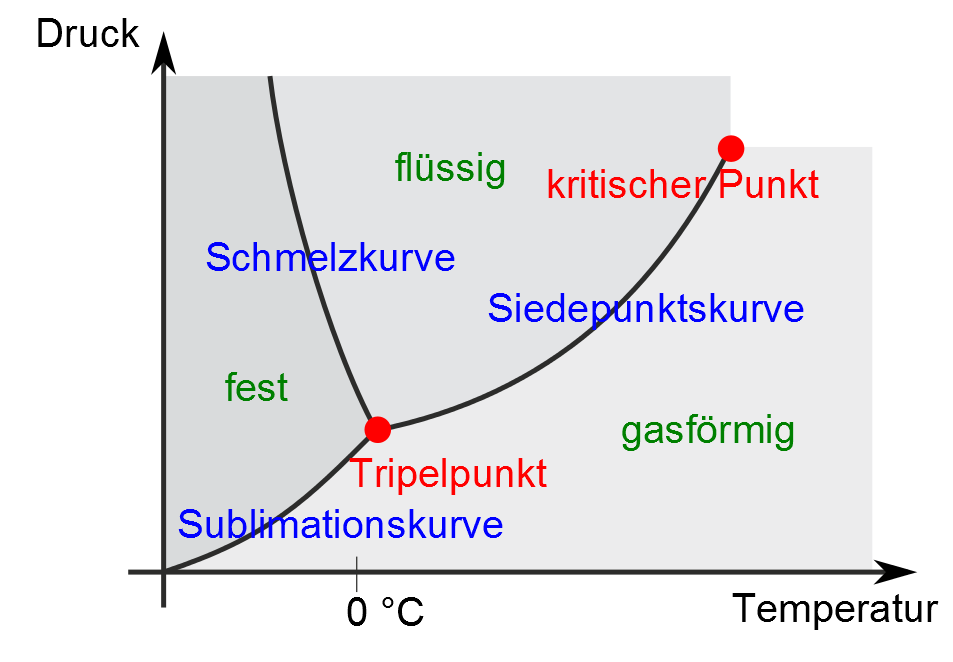
\includegraphics[width=\textwidth]{Bilder/aggregatzustand.png}
        \caption{Phasendiagramm Wasser}
    \end{minipage}
    \hfill
    \label{fig:Phasendiagramm}
\end{figure}